\section{Methodology}\label{sec:methodology}
This section will provide an overview of different types of Decision Diagrams, how they each are structured, their differences and how they can be converted from one to another.

The different approaches that can be taken for the Baum-Welch algorithm will also be discussed, including the recursive, matrix-based, and \gls{add}-based approaches. The advantages and limitations of each approach will be highlighted.

Finally, the \gls{cudd} library will be introduced, which is a library for implementing and manipulating \glspl{bdd} and \glspl{add}.

\subsection{Decision Diagrams}\label{subsec:decision-diagrams}
\acrfullpl{bdd} are data structures for efficiently representing and manipulating Boolean functions.
They are a compressed representation of truth tables, capturing the logical structure of a function in a graph-based format by eliminating redundancy, reducing memory usage, and improving computational efficiency~\cite{bryant1986graph}.

A \gls{bdd} is a directed acyclic graph derived from a decision tree, where each non-terminal node represents a Boolean variable, edges correspond to binary assignments (0 or 1), and terminal nodes store function values (0 or 1).
To reduce the size of the decision tree, \glspl{bdd} exploit redundancy by merging equivalent substructures, resulting in a canonical form (when reduced and ordered) that allows for efficient operations such as function evaluation, equivalence checking, and Boolean operations~\cite{bryant1986graph}.

\glspl{bdd} have been widely used in formal verification, model checking, and logic synthesis due to their ability to compactly represent large Boolean functions while maintaining efficient computational properties.
However, in rare cases \glspl{bdd} can suffer from exponential blowup. This can occur particularly when dealing with functions that lack inherent structure or when representing numerical computations that go beyond Boolean logic.

\subsection{ADDs}\label{subsec:adds}
\acrfullpl{add} generalize the concept of \glspl{bdd} by allowing terminal nodes to take values beyond Boolean constants (0 and 1).
Instead of restricting values to true/false, \glspl{add} can store arbitrary numerical values, making them useful for representing and manipulating functions over discrete domains~\cite{bahar1997algebric}.
This generalization enables the efficient representation of functions such as cost functions~\cite{kwiatkowska2004probabilistic}, probabilities~\cite{baier1997symbolic}, and other numerical relationships that arise in probabilistic reasoning.

The fundamental structure of an \gls{add} remains similar to a \gls{bdd}, where a decision tree is compacted by merging redundant substructures.
However, instead of performing Boolean operations, \glspl{add} allow for arithmetic operations such as addition and multiplication, making them well-suited for applications like dynamic programming, \glspl{mdp}, and linear algebraic computations~\cite{bahar1997algebric}.

\subsection{Recursive vs. Matrix vs. ADD-based Approaches}\label{subsec:approaches}
When working with the Baum-Welch algorithm, different approaches can be taken to optimize computational efficiency.
Three common strategies are recursive, matrix-based, and \gls{add}-based approaches, each with distinct advantages and limitations.


\begin{itemize}
    \item \textbf{Recursive Approach:} Conceptually simple, recursion follows a divide-and-conquer strategy, and makes use of a dynamic programming approach. Previous calculations are used to build upon future calculations. These results are stored in a list or a map, so that they can be accessed when needed ~\cite[Chapter 4]{cormen2022introduction}.
    \item \textbf{Matrix Representation:} Reformulating algorithms using matrix operations leverages algebraic properties for parallel computation and efficient processing.
          By building upon the recursive approach, matrices provide an efficient method of accessing the stored results leading the faster computations overall~\cite[Chapter 4, 15 \& 28]{cormen2022introduction}.
    \item \textbf{ADD-based Approach:} \glspl{add} provide a compact representation that eliminates redundancy in recursive computations.
          By reusing previously computed substructures, they improve efficiency and reduce memory overhead~\cite{bahar1997algebric}.
          Compared to matrices, \glspl{add} can offer a more space-efficient alternative for structured data while extending \gls{bdd} techniques to handle both Boolean and numerical computations.
\end{itemize}


In this work we explore the benefits of \gls{add}-based approaches for solving complex problems, focusing on parameter estimation in \glspl{dtmc} and \glspl{ctmc}.
We compare the performance of \gls{add}-based algorithms against recursive-based implementations, highlighting the advantages of using \glspl{add} for efficient computation and memory management.

\subsection{CuDD}\label{subsec:cudd}
\acrfull{cudd} is a library for implementing and manipulating \glspl{bdd} and \glspl{add} developed at the University of Colorado.
The \gls{cudd} library~\cite{somenzi1997cudd} is a powerful tool for implementing and manipulating decision diagrams, including \glspl{bdd} and \glspl{add}.

Implemented in C, the \gls{cudd} library ensures high-performance execution and can be seamlessly integrated into C++ programs, which we utilize in this paper.
By leveraging the \gls{cudd} library, we demonstrate the benefits of \gls{add}-based approaches for solving parameter estimation problems in \glspl{dtmc} and \glspl{ctmc}.

In this project, we use the \gls{cudd} library to store \glspl{add} and perform operations on them.
Its optimized algorithms and efficient memory management enable symbolic handling of large and complex matrices, significantly improving performance compared to traditional methods.



\subsection{From Prism to CuPAAL}\label{subsec:from_prism_to_cupaal}
The models are encoded from Prism models to CuPAAL models. This is done by parsing the Prism model to Jajapy, using Stormpy.

The Jajapy model contains a matrix for it's transitions, a matrix for it's labels, and a vector for the initial state.
The model is passed to CuPAAL where these matrices and vectors are encoded into \glspl{add}, as a function $f \colon {0,1}^n \times {0,1}^n \to R$.

The Transition matrix is a $S\times S$ matrix, where $S=States$, and is encoded to an \gls{add}, by each row and column with a binary value. This value is determined based on the size of the matrix,
$n = \ceil{log_2(S)}$.

The label matrix is a $S\times L$ matrix, where $L=Labels$ and since there is no guarantee that $S = L$, the encoding is handled differently.
The matrix is instead treated as a list of vectors.
Each vector is encoded as square matrices, where each row or column (depending on the vector type) is duplicated, which is then encoded to a list of \glspl{add}.
Knowing the exact dimensions of matrices and that they are square helps to simplify some of the symbolic operations.
An example of this will be displayed in \autoref{subsec:kronecker-product-implementation}.

The Initial state vector is encoded similarly to the label matrix, but only as a single \gls{add}.

We have not modified or extended the CUDD library.
All functionality used in our implementation is available through the standard CUDD library.


\subsection{Kronecker Product Implementation}\label{subsec:kronecker-product-implementation}
This section will provide an overview of how the Kronecker product is implemented in CuPAAL, using the row and column duplication method mentioned in \autoref{subsec:from_prism_to_cupaal}.

The structure of Decision Diagrams in CuPAAL, where keeping track of all the new binary values used for encoding from a matrix to an \gls{add} can add a layer of complexity for calculation.
Especially when computing operations that translate matrices to new dimensions, such as the Kronecker product.
This matrix-based approach enables efficient symbolic operations, as the Kronecker product can be calculated by taking the Hadamard product between a column matrix \gls{add} and a row matrix \gls{add}, simplifying what would otherwise be a more complex operation.

An example of this can be seen with the two vectors $\hat{A}$ and $\hat{B}$

Let $\hat{A} = \begin{bmatrix}
        1 \\
        2
    \end{bmatrix}$
and $\hat{B}=\begin{bmatrix}
        3 & 4
    \end{bmatrix}$.

The Kronecker product of these two vectors is computed as follows:
\begin{equation}
    \hat{A} \otimes \hat{B} = \begin{bmatrix}
        1 \cdot 3 & 1 \cdot 4 \\
        2 \cdot 3 & 2 \cdot 4
    \end{bmatrix} = \begin{bmatrix}
        3 & 4 \\
        6 & 8
    \end{bmatrix}.
    \label{eq:kronecker-product-example}
\end{equation}

Another way to calculate the Kronecker product is to expand the vectors into matrices.
$\hat{A}$ and $\hat{B}$ are expanded to be matrices, similar to how the matrix was treated as a list of vectors and then expanded to square matrices, as seen with the Label matrix.

Let $\mathbf{A} = \begin{bmatrix}
        1 & 1 \\
        2 & 2
    \end{bmatrix}$ and
$\mathbf{B} = \begin{bmatrix}
        3 & 4 \\
        3 & 4
    \end{bmatrix}$.

The Kronecker product of $\hat{A}$ and $\hat{B}$ can also be calculated, by using the Hadamard product of $\mathbf{A}$ and $\mathbf{B}$.
This is done as follows:


\begin{equation}
    \mathbf{A} \circ \mathbf{B} = \begin{bmatrix}
        1 \cdot 3 & 1 \cdot 4 \\
        2 \cdot 3 & 2 \cdot 4
    \end{bmatrix} = \begin{bmatrix}
        3 & 4 \\
        6 & 8
    \end{bmatrix}.
\end{equation}


Hereby showing that the Hadamard product can be used to compute the Kronecker product between two matrices, by using the row and column duplication method.


\subsection{Implementation to Jajapy}\label{subsec:implementation-to-jajapy}
This section will give an overview of how \Cupaal\ is implemented into \Jajapy, using bindings between C++ and Python.
\autoref{fig:cupaal-jajapy-architecture} shows the overall architecture of the implementation.


\begin{figure}[htb!]
    \centering
    \usetikzlibrary{shapes.geometric, arrows, fit, calc, automata, positioning, tikzmark,chains, scopes}
%%% done
% Events
\usetikzlibrary{shapes.multipart}
\tikzstyle{arrow} = [thick,->,>=stealth]

\tikzstyle{state} = [rectangle, minimum width=2cm, minimum height=0.7cm, text centered, draw=black, fill=white!30, align=center]
\tikzstyle{cluster} = [line width=0.4pt, draw=black, inner sep=0.5em, rounded corners=0.1cm]
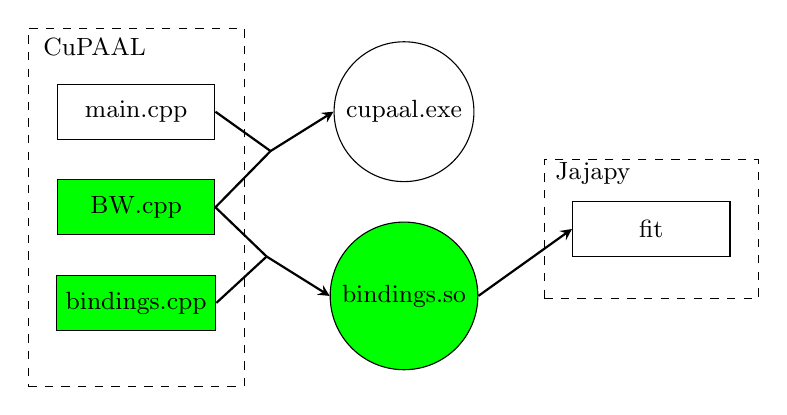
\begin{tikzpicture}[start chain=1 going below,
        start chain=2 going below,
        node distance=.5cm and 1.5cm,
        roundnode/.style={circle, minimum size=7mm, text centered, draw=black, fill=white!30, align=center},
        every node/.style={font=\small}]

    \node [on chain=1, state] (trainingset) {main.cpp} node[below,scale=1, xshift=-15,yshift=30]{CuPAAL};
    \node [on chain=1, state, fill=green] (learning) {BW.cpp};
    \node [on chain=1, state, fill=green] (bind) {bindings.cpp};

    \node [on chain=2, roundnode, right=of trainingset] (cupaal) {cupaal.exe};
    \node [on chain=2, roundnode, fill=green] (bindings) {bindings.so};
    \node [below right=of cupaal, state] (candice) {fit} node[below,scale=1, xshift=165,yshift=-15]{Jajapy};

    \node[draw, dashed, fit={(trainingset) (learning) (bind)},
        inner xsep=10pt, inner ysep=20pt] (box1) {};
    \node[draw, dashed, fit={(candice)},
        inner xsep=10pt, inner ysep=15pt] (box1) {};
    \coordinate (Qf) at ([xshift=-0.8cm, yshift=-0.5cm]cupaal.west);
    \coordinate (Qg) at ([xshift=-0.8cm, yshift=0.5cm]bindings.west);

    \draw[arrow, -] (trainingset.east) --  (Qf);
    \draw[arrow, -] (learning.east) --  (Qf);
    \draw[arrow, -] (bind.east) --  (Qg);
    \draw[arrow, -] (learning.east) --  (Qg);
    \draw[arrow, ->] (Qf) -- (cupaal.west);
    \draw[arrow, ->] (Qg) -- (bindings.west);
    \draw[arrow, ->] (bindings.east) -- (candice.west);
\end{tikzpicture}
    \caption{Architecture of \Cupaal\ combined with \Jajapy.}
    \label{fig:cupaal-jajapy-architecture}
\end{figure}


\Cupaal\ consists of two main componenets, the main function and the \gls{bw} library.
Both of these are compiled to an executable program, called \texttt{cupaal.exe}, which can be used to run the Baum-Welch algorithm on a given model.

To implement \Cupaal\ into \Jajapy, we create bindings between C++ and Python using the \texttt{pybind11} library~\cite{pybind11github}.
This allows us to call C++ functions from Python, enabling us to use \Cupaal\ in \Jajapy.

We create a C++ bindings file, that uses the \gls{bw} library from \Cupaal\ and defines the function we want to expose to Python, we call this function $cupaal\_bw\_symbolic$, seen in~\autoref{lst:cupaal-bindings}.
This function takes model parameters from a \Jajapy\ model as input, and transforms them to be used in \Cupaal.


\begin{listing}[htb!]
    \begin{minted}{cpp}
// Some parameters have been removed for brevity
cupaal_markov_model cupaal_bw_symbolic(vector<string>& states, vector<string>& labels, vector<vector<string>>& observations, vector<double>& initial_distribution, vector<double>& transitions, vector<double>& emissions, int max_iterations = 100, double epsilon = 1e-2){
    MarkovModel model(states, labels, initial_distribution, transitions, emissions, observations);
    cupaal_markov_model model_data;
    chrono::seconds time = chrono::seconds(3600);
    model.baum_welch_multiple_observations(
        max_iterations, epsilon, time);

    // Removed output and result path for brevity
    model_data.initial_distribution = model.initial_distribution;
    model_data.transitions = model.transitions;
    model_data.emissions = model.emissions;
    
    Cudd_Quit(model.manager);
    return model_data;
}
      \end{minted}
    \caption{C++ bindings file for CuPAAL}
    \label{lst:cupaal-bindings}
\end{listing}


\autoref{lst:cupaal-bindings} calculates the Baum-Welch algorithm using~\autoref{lst:baum-welch-multiple-observations} from \Cupaal, and returns the results to Jajapy, as a tuple with the relevant values.
These being the initial distribution, the transitions and the emissions.


\begin{listing}[htb!]
    \begin{minted}{cpp}
        void baum_welch_multiple_observations(unsigned int max_iterations = 100, double epsilon = 1e-6, chrono::seconds time = chrono::seconds(3600));
        \end{minted}
    \caption{Prototype of the function used to run the Baum-Welch algorithm on multiple observations in CuPAAL.}
    \label{lst:baum-welch-multiple-observations}
\end{listing}


The C++ bindings file is then compiled to a shared library, which can be imported in Jajapy.
Jajapy can call the $cupaal\_bw\_symbolic$ function, which will then call the CuPAAL implementation of the Baum-Welch algorithm.

We create a new function in Jajapy, called \texttt{\_bw\_symbolic}, which is used to call the \Cupaal\ implementation of the Baum-Welch algorithm, as seen in~\autoref{lst:jajapy-bw-symbolic}.


\begin{listing}[htb!]
    \begin{minted}{python}
def _bw_symbolic(self, max_iteration = 100, epsilon = 1e-2, outputPath = "", resultPath = ""):
    try:
        import libcupaal_bindings
    except ModuleNotFoundError:
        print("Cannot find module")

    states = [str(i) for i in range (self.h.nb_states)]
    labels = list(set(self.h.labelling))
    observations = []
    for times, sequences in zip(self.training_set.times, self.training_set.sequences):
        for i in range(times):
            observations.append(list(sequences))
    initial_state = self.h.initial_state.tolist()
    transitions = self.h.matrix.flatten().tolist()
    emissions = zeros((len(labels), self.h.nb_states))
    for row in range(len(labels)):
        for col in range(self.h.nb_states):
            if self.h.labelling[col] == labels[row]:
                emissions[row][col] = 1
    emissions = emissions.flatten().tolist()

    cupaal_model = libcupaal_bindings.cupaal_bw_symbolic( states, labels, observations, initial_state, transitions, emissions, max_iteration, epsilon, outputPath, resultPath)
    self.h.initial_state = array(cupaal_model.initial_distribution)
    self.h.matrix = array(cupaal_model.transitions).reshape( self.h.nb_states, self.h.nb_states)
    self.h.emissions = array(cupaal_model.emissions).reshape( len(labels), self.h.nb_states)
    return self.h
      \end{minted}
    \caption{Jajapy's implementation of the Baum-Welch algorithm using CuPAAL.}
    \label{lst:jajapy-bw-symbolic}
\end{listing}


The fit function in Jajapy is modified to call the \texttt{\_bw\_symbolic} function when a new parameter called \texttt{symbolic} is set to true, as seen in~\autoref{lst:jajapy-fit-cupaal}.


\begin{listing}[htb!]
    \begin{minted}{python}
# Some parameters have been removed for brevity
def fit(self, output_file: str, output_file_prism: str, epsilon: float, max_it: int, symbolic: bool):
    # Removed preparation and settings number of processes, for brevity
    if symbolic :
        return self._bw_symbolic(max_it, epsilon, output_file, output_file_prism)
    else:
        return self._bw(max_it, pp, epsilon, output_file, output_file_prism, verbose, stormpy_output, return_data)
      \end{minted}
    \caption{Jajapy's fit function, which calls the CuPAAL implementation of the Baum-Welch algorithm when symbolic is set to true.}
    \label{lst:jajapy-fit-cupaal}
\end{listing}


When the parameter is true, the Jajapy model will call the~\autoref{lst:jajapy-bw-symbolic} function, which will then call the CuPAAL implementation of the Baum-Welch algorithm.




